\documentclass[12pt, oneside]{book}

\usepackage{graphicx}  % this is for includegraphics
\graphicspath{{figures/}}

\usepackage{setspace}
\onehalfspacing % this sets spacing to 1.5 

\usepackage{subfig}
\usepackage{amsmath}
\usepackage{amsthm} % for theorems, lemmas etc
\usepackage{amsfonts}
\usepackage{lipsum} % to generate the lipsum random text in the sample
\usepackage{tikz}
\usepackage{siunitx}
\usetikzlibrary{calc,decorations.pathmorphing,patterns}


\usepackage[colorlinks=true, urlcolor=blue, pdfborder={0 0 0}]{hyperref}
\hypersetup{
     colorlinks   = true,
     citecolor    = blue
}

\theoremstyle{plain}
\newtheorem{theorem}{Theorem}[section]
\newtheorem{proposition}[theorem]{Proposition}
\newtheorem{lemma}[theorem]{Lemma}
\newtheorem{corollary}[theorem]{Corollary}
\newtheorem{fact}[theorem]{Fact}

\theoremstyle{definition}
\newtheorem{definition}[theorem]{Definition}
\newtheorem{example}[theorem]{Example}
\newtheorem{remark}[theorem]{Remark}
\newtheorem{remarks}[theorem]{Remarks}

\newcommand{\Cov}{\mathrm{Cov}}
\newcommand{\Var}{\mathrm{Var}}

\begin{document}

\begin{titlepage}
\begin{center}
        \vspace{-2cm}
Mathematical Finance MSc Dissertation MTH775P, 2018/19 
		\\
        \Huge
        \textbf{Accelerated Grids}
        \\        
        \vspace{0.4cm}
        \LARGE
        Optimizing Solvers for Financial Partial Differential Equations
        \\        
        \vspace{0.4cm}        
        \textbf{Mustafa Berke Erdis, ID 180883925}% student name and number        
        \\
        \large Supervisor: Dr. Sebastian del Bano Rollin
        \\
        \vspace{0.9cm}
        
\includegraphics[scale=0.23]{QMCrest.png}
        \\
        \vspace{0.9cm}        
        \LARGE 
        A thesis presented for the degree of\\
        Master in Sciences in \emph{Mathematical Finance}\\
        \vspace{0.7cm}        
        \Large
        School of Mathematical Sciences\\ 
        and \emph{School of Economics and Finance}\\
        Queen Mary University of London \\
    \end{center}
\end{titlepage}


\chapter*{Declaration of original work}
\begin{flushright}
This declaration is made on \today.
\end{flushright}


{\bf Student's Declaration:}
I, Mustafa Berke Erdis, hereby declare that the work in this thesis 
is my original work. I have not copied from any other students' work, work of 
mine submitted elsewhere,  or from any other sources except where due reference or acknowledgement is made explicitly in the text, nor has any part been written for me by another person.

Referenced text has been flagged by:
\begin{enumerate}
\item Using italic fonts, {\bf and} % LaTeX: {\it text}  
\item using quotation marks ``\ldots '', {\bf and}
\item explicitly mentioning the source in the text.
\end{enumerate}

%This excludes any definitions known from your modules or undethat can be found in an undergraduate text book.

\newpage

\thispagestyle{empty}
        \begin{flushright}
                This work is dedicated to my family.
        \end{flushright}
\vspace{\stretch{2}}\null



\chapter*{Acknowledgements}
Here you thank people that have helped you in the journey. \\
\lipsum[100] % replace this by your text

\chapter*{Abstract}
\begin{center}
\small 
Here you write a short summary, around 10 lines, of your work. \\
\lipsum[100]% replace this by your text
\end{center}       


\chapter*{Preface}
Here  you write a summary of the work. A paragraph on the motivation, previous work, then maybe a brief chapter by chapter summary. 

\lipsum[100]% replace this by your text

\begin{flushright}
Queen Mary University of London\\
12${}^{\text{th}}$ August 2019
\end{flushright}

\tableofcontents

\chapter{Introduction}
In Ancient Greece, Thales was scorned for his poverty. Later that year, Thales utilized his skills in astrology to forecast an increase in olive yields. Using his limited capital, he rented oil presses in winter. Months later, over the oil making season, many people rushed to the presses because of the high yields that Thales predicted. As he rented the presses over the winter, he forced the terms he pleased. Thales showed it was easy for philosophers to be rich if they chose it and practically used the first  financial derivative product \cite{thalesians}. 

In the modern world, financial derivatives are contracts between two or more parties. The value of the contract depends on one or several underlying assets. Commonly the assets are currencies, equities, bonds, interest rates, market indices or commodities. The vanilla call option gives the right but not the obligation to buy the underlying asset at the expiry date at a previously agreed strike price. Essentially, Thales bought call options for oil presses.  If the olive yields didn't come as Thales expected he didn't have the obligation to use the olive presses.  On the other hand, the vanilla put option gives the right but not the obligation to sell the underlying asset at the expiry date at a previously agreed strike price. Practical applications of the options include hedging or speculating the future asset price. Hence, accurately pricing the options is crucial for an efficient and mature financial market.

Merton and Scholes received the 1997 Nobel Prize in Economic Science for this work \cite{merton}. 

\section{Motivation of the Project}
Derivative pricing in the real world is a computationally intensive task. The existing numerical methods for partial differential equations are all constrained by the computational complexity. Being fast when evaluating new information is critical for the operations of hedge funds and investment banks. Therefore optimizing the existing numerical methods with hardware and software that can be installed on a trading floor is crucial. Goal of the project is to provide efficient methods for pricing options.

Purpose of this project to optimize numerical solutions of parabolic PDEs by testing high performance computing techniques and comparing compilers/os/32bit/64bit.
The idea of this project is to study how to take advantage of this parallelism and explore how much faster we can make these calculations.

\section{Literature Review}
Bakılacak paperlar ekle.

\section{Contents of the Thesis}
Included in your ‘Introduction’ section should be a clear summary of  what  you  have  achieved  in  the  project  work  presented,  such  as  any  new  results, generalisations, corollaries, examples, new connections, or computer investigations.  The thesis is organized as follows.  Chapter 2 presents an introduction to financial derivatives, Black-Scholes model and finite difference models.  Chapter3 extends the 2d and gives examples of two dimensional heat equation.  Chapter 4 develops the numerical methods and techniques considered to solve the PDE-based models for the option pricing problems.  In the same chapter,  finite difference method with improved algorithms to solve a large tridiagonal systems is discussed.  Chapter 5 shows the numerical results of our numerical methods with several examples of.  Chapter 6 concludes the thesis.

\chapter{Pricing Financial Derivatives}\label{Pricing Financial Derivatives}
\section{The Risk Neutral Approach}
The Black-Scholes framework is a theoretical valuation formula for options. It reveals the relationship between the prices of the options and the underlying assets. Since almost all corporate liabilities can be viewed as combinations of options, the formula is applicable to common stocks and corporate bonds \cite{BS}. The Black-Scholes model makes the following assumptions:
\begin{itemize}
\item There does not exist any arbitrage opportunity in the financial market.  The traders can’t make instantaneous profit without any risk.
\item The underlying asset value follows a geometric Brownian Motion $dS = \mu S dt + \sigma S dB $ where $\mu$ denotes the average rate of growth of the underlying assets, $\sigma$ denotes the volatility of the asset price and B is a Brownian Motion.
\item The market is frictionless.  This means there are no transaction fees, the interest rates for borrowing and lending money from and to the bank are the same, every party  in  market  has  immediate  information  and  all  entities  are  available  at  anytime and in any size.
\item No dividend will paid on the underlying asset $S$.
\end{itemize}

\subsection{Black-Scholes Partial Differential Equation}
The original model is used to price the vanilla  option, which is the simplest type of option.
Under the assumptions of Black-Scholes framework, the call or put option price satisfies the parabolic partial differential equation:

\begin{equation}
\frac{\partial V}{\partial t} = rS\frac{\partial V}{\partial S}+\frac{1}{2} \sigma^2 S^2 \frac{\partial^2 V}{\partial S^2} - rV
\end{equation}

Framework shows the  price V(t,S)  of  a  European  option  driven  by  one underlying asset that satisfies the PDE where $r$, $\sigma$, $t$, $S$respectively denotes the risk-free interest rate, volatility, time and the underlying price.  It is assumed that $r$ and $\sigma$ are constants. In more complicated models such as stochastic volatility models they can be a function. In order to price a vanilla call option the PDE needs to satisfy the following boundary and initial conditions.

\begin{eqnarray}
C(0,t) &=& 0, \hspace{4pt} C(S_{\max},t)=S_{\max} - K e^{-r(T-t)}, \hspace{10pt} 0 \leq t \leq T \\[10pt]
C(S,T) &=& \max(S-K,0), \hspace{10pt} 0 \leq S \leq S_{\max}
\end{eqnarray}

\subsection{Derivation of the Black-Scholes Equation}
Black-Scholes model takes advantage of the properties of the geometric Brownian motion and It\^{o}'s lemma. 

\begin{definition} Brownian Motion 
Brownian motion (also known as Wiener Process) was discovered by botanist Robert Brown as he observed a chaotic motion of particles suspended in water \cite{BM}. A  Brownian  motion, $B(t)$,  is  a  continuous-time  stochastic  process  with  the  following properties: 
\begin{itemize}
\item $ B(0) = 0 $.
\item $ B(t) $ is a continuous function of t.
\item For $ 0  \leq s < t $ the increment $ B(t) -  B(s)  $ has normal distribution $ \mathcal{N}(0, t-s) $.
\end{itemize}
Brownian motion is the basic building block in stochastic calculus and geometric Brownian motion is used to model the stock prices in Black-Scholes model.
\end{definition}

\begin{lemma} It\^{o}'s Lemma
Let $B(t)$ be a Brownian motion and $X(t)$ be an Ito process which satisfies the stochastic differential equation:
\begin{equation}
dX(t) = \mu(X(t),t)dt + \sigma(X(t),t)dB(t)
\end{equation} 
If $f(x, t) \in C^2(\mathbb{R}^2,\mathbb{R})$ then $f(X(t),t)$ is also an Ito drift-diffusion process, with its differential given by:
\begin{equation}
d(f(X(t),t)) = \frac{\partial f}{\partial t}(X(t),t)dt + f'(X(t),t)dX + \frac{1}{2}f''(X(t),t)dX(t)^2
\end{equation} 
With $dX(t)^2$ given by: $dt^2 = 0$, $dt dB(t) = 0$ and $dB(t)^2 = dt$.
\end{lemma}

\begin{theorem}
Assume that the asset price $S$ follows a geometric Brownian motion.  Under the assumptions of Black-Scholes framework, the call or put option price $V(t,S)$ satisfies the parabolic partial differential equation
\begin{equation}
\frac{\partial V}{\partial t} = rS\frac{\partial V}{\partial S}+\frac{1}{2} \sigma^2 S^2 \frac{\partial^2 V}{\partial S^2} - rV
\end{equation}
\end{theorem}

\begin{proof}
Suppose an investor sets up a self-financing portfolio,  $ X(t)$, comprising one option and an $\Delta$ amount of the underlying asset. Therefore, value of the portfolio at time t is $X(t) = V(t) + \Delta S(t)$. 
Since the self-financing trading strategy has no capital influx or consumption, the value of portfolio change can be written as 
\begin{equation}
dX = dV + \Delta dS
\end{equation}

Applying the It\^{o}'s Lemma to the option price V(t,S)
\begin{equation}
dV = \frac{\partial V}{\partial t} dt + \frac{\partial V}{\partial S} (S,t) dS + \frac{1}{2}\frac{\partial^2 V}{\partial S^2}(S,t)dS^2
\end{equation}

Since the Black-Scholes model assumes that the stock price under the "market probability measure" follows a gBM. 
\begin{equation}
dS = \mu S dt + \sigma S dW
\end{equation}

Putting (1.4) and (1.6) together yields
\begin{equation}
dV = (\frac{\partial V}{\partial t} + \mu S \frac{\partial V}{\partial S} + \frac{1}{2} \sigma^2 S^2 \frac{\partial^2 V}{\partial S^2} + \Delta \mu S) dt + (\sigma S \frac{\partial V}{\partial S}+\Delta \sigma S) dW
\end{equation}

The fact that portfolio is risk-free implies that the second term involving the Brownian Motion, $dW$, must be zero.  This technique is known as delta-hedging , otherwise, we would have an arbitrage opportunity. Thus, $ \Delta = - \frac{\partial V}{\partial S}$.  Hence, the growth rate of the portfolio must be the risk free rate which can be summarized as $ dX = r X dt $. Substituting $\Delta$ and $dX$ yields

\begin{equation}
\frac{\partial V}{\partial t} + \frac{1}{2} \sigma^2 S^2 \frac{\partial^2 V}{\partial S^2} = r(V-S\frac{\partial V}{\partial S})
\end{equation}

Rearranging the equation to get famous Black-Scholes equation:
\begin{equation}
\frac{\partial V}{\partial t} = rS\frac{\partial V}{\partial S}+\frac{1}{2} \sigma^2 S^2 \frac{\partial^2 V}{\partial S^2} - rV
\end{equation}
\end{proof} 

\begin{definition} The resulting partial differential equation can be solved analytically using the following boundary conditions and initial conditions for call options.
\begin{eqnarray}
\frac{\partial C}{\partial t} &=& rS\frac{\partial C}{\partial S}+\frac{1}{2} \sigma^2 S^2 \frac{\partial^2 C}{\partial S^2} - rC \\[10pt]
C(0,t) &=& 0, \hspace{4pt} C(S_{\max},t)=S_{\max} - K e^{-r(T-t)}, \hspace{10pt} 0 \leq t \leq T \\[10pt]
C(S,T) &=& \max(S-K,0), \hspace{10pt} 0 \leq S \leq S_{\max}
\end{eqnarray}

Solving the equations, the formulae \cite{wilmott} for European call is
\begin{eqnarray}
C = S \Phi (d_1) - K e^{-r(T-t)} \Phi (d_2) \\[10pt]
d_1 = \frac{log(S/K) + (r + \sigma^2/2)(T - t)}{\sigma \sqrt{T-t}} \\[10pt]
d_2 = d_1 - \sigma \sqrt{T-t}
\end{eqnarray}

\end{definition}

\begin{remark}  Untradable assets\\ 
Modern financial engineering created derivatives using untradable assets as an underlying such as multi asset derivatives like equity baskets, weather derivatives and non-deliverable forwards. Non-deliverable forwards are for offshore investors that want to trade non-convertible currencies such as Brazilian Real, South Korean Won.  The Black-Scholes model is still used in these cases \cite{weather} \cite{basket} but not entirely applicable to assets that cannot be hedged.
\end{remark}


\section{Solving Partial Differential Equations}
Since the foundation of the world humanity tried to understand and model the nature. Differential equations serves this purpose by enabling us to describe natural phenomena for instance, heat, sound and fluid flow. General form of 2nd order PDEs of two independent variables is $$ au_{xx} + bu_{xy} + cu_{yy} + du_x + eu_y + fu + g = 0 $$ If the equation satisfies the condition $ b^2 - 4ac = 0 $  it is considered a parabolic partial differential equation. Generally, financial partial differential equations can be classified as parabolic partial differential equations.

Generally, partial differential equations are too complicated to work out an analytical solution. Thus, we need to achieve a numerical solution to the problem. Numerical partial differential equations includes components in the areas of applications, mathematics and computers. The most common framework is finite difference method which tries to find approximate solutions to the problem at a discrete set of points, normally on a rectangular grid of points. Instead we try to find approximate solutions of the problem at a discrete set of points in the (x, t) plane, normally a rectangular grid of points. It is simple to construct and analyse but can compromise performance because of increased computational complexity when there are high dimensions. 

Multidimensional finite differences (such as ADI schemes) are only practical up to 3 dimensions, higher dimension are too demanding in terms of computer memory and computing time.

For higher order problems Monte Carlo is usually the method of choice. Using low discrepancy quasi random suites (e.g. Sobol) along with the Brownian bridge technique leads to reasonable computing times. See for instance Jaeckel's book "monte carlo methods in finance".

Feynman-Kac theorem \cite{klebaner}, establishes a link between parabolic partial differential equations and stochastic processes by writing the solution as a conditional expectation. Thanks to the theorem, Monte Carlo method is also utilized to find the numerical solutions to the partial differential equations.  Monte Carlo method is preferred when the dimensions are too high !!Glassermann MC book rough calculation of error MC vs PDE grids(1-2 pages)!!

The finite difference method has become a very popular for approximating the Black Scholes equation. This equation is an example of a convection-diffusion equation. Heat equation is the most basic convection-diffusion equation, we will be using it as a benchmark to test the methods. 

\subsection{Heat Equation}
Most basic case for parabolic differential equations is the heat equation. In the experiments the following initial and boundary conditions will be used.

\begin{eqnarray}
u_t(x,t) &=& u_{xx}(x, t) \\[10pt]
u(0, t) &=& u(x_{max}, t) = 0, \hspace{10pt} 0 \leq t \leq T \\[10pt]
u(x, 0) &=& sin(\pi x), \hspace{10pt} 0 \leq x \leq x_{\max}
\end{eqnarray}

\begin{definition} Analytical Solution of Heat Equation

Certain kinds of partial differential equations allows us to find an analytical solution with the help of the Separation of Variables technique \cite{duffyfinite}.

\begin{eqnarray}
u(x,t) = X(x) T(t) \\[10pt]
u_{xx}(x, t) = X^{''}(x) T(t) \\[10pt]
u_t (x,t) = X(t) T^{'}(t)
\end{eqnarray}

Using the partial derivatives the equation $ u_t = u_{xx} $ becomes
\begin{equation}
\frac{T^{'}(t)}{T(t)}  = \frac{X^{''}(x)}{X(x)}
\end{equation}

Right hand side only depends on x and the left hand side depends only on t. Therefore, the equation is valid only when each side is equal to a constant, which we set to $ \lambda $. Rearranging terms gives us the following equations:

\begin{eqnarray}
\frac{T^{'}(t)}{T(t)}  = \frac{X^{''}(x)}{X(x)} = \lambda \\[10pt]
X^{''}(x) = \lambda X(x), \hspace{10pt} T^{'}(t) = \lambda T(t) \\[10pt]
X(0) = X(1) = 0
\end{eqnarray}

Solving for X(x) is an example case of Sturm-Liouville problem \cite{sepvar}. However the $\lambda < 0$ and $\lambda = 0$ cases result in trivial solutions, thus they are discarded. Solving for $\lambda > 0$ yields
\begin{equation}
X(x)= c_1 sin(kx) + c_2 cos(kx)
\end{equation}

The boundary conditions leads to $ c_2 = 0, c_1 sin(k) = 0 \rightarrow k = 0, \pi, 2\pi, ...n\pi$ where n is an integer.

Solving for $T(t)$ gives the solution
\begin{eqnarray}
T(t) = c_3 exp(-n^2 \pi ^2 t) \\[10pt]
u(x,t) = \sum_{n=1}^{\infty} b_n exp(-n^2 \pi ^2 t) sin(n \pi x)
\end{eqnarray}

where we have set $b_n = c_1 c_3$. The initial condition gives
\begin{equation}
u(x,0) = sin(\pi x) = \sum_{n=1}^{\infty} b_n sin(n \pi x)
\end{equation}
which is a Fourier sine series. Thus, the coefficient $b_n$ is chosen such that
\begin{equation}
b_n = 2 \int_{0}^{1} sin(\pi x) sin(\pi n x) dx = \frac{2sin(\pi n)}{\pi - \pi n^2}
\end{equation}
Combining the solutions
\begin{equation}
u_n(x,t) = \sum_{n=1}^{\infty} \frac{2sin(\pi n)}{\pi - \pi n^2} exp(-n^2 \pi ^2 t) sin(n \pi x)= exp(-\pi t) sin(\pi x)
\end{equation}
\end{definition}

\section{Finite Difference Methods}
\subsection{Discretization}
Essentially, solving a PDE is the problem of finding a function which depends on values at infinitely many points. Naturally, the finite difference methods first step is to make the problem discrete that we are able to solve \cite{jwthomas}. As a result, we need to discretise the space dimensions and time dimension. The discretization procedure begins by replacing the domain $[0, x_{max}]$ x  $[0, T]$  by a set of mesh points. In order to get a $n$ x $m$ equally spaced mesh points the step sizes are calculated as $ \Delta t = \frac{T}{m}$, $\Delta x = \frac{x_{max}}{n}$.

\begin{figure}[!htb]
    \centering
        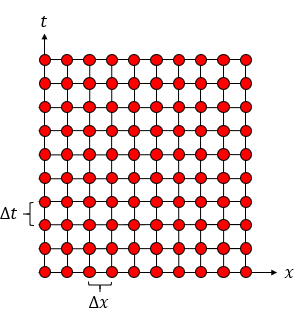
\includegraphics[scale=0.8]{Discretize.png}
    \caption{10 x 10 grid.}
\end{figure}
In order to replace our PDE, we need to utilize finite difference approximations for the partial derivatives. Notationally, we will define $u^n_i$ to be a function defined at the point $(i \Delta x, n \Delta t) $.

\begin{itemize}
        \item Forward difference: $ \frac{\partial u}{\partial t} = \frac{u^{n+1}_i - u^n_i}{\Delta t} $
        \item Central difference: $ \frac{\partial u}{\partial t} = \frac{u^{n+1}_i - u^{n-1}_i}{\Delta t} $
        \item Backwards difference: $ \frac{\partial u}{\partial t} = \frac{u^{n}_i - u^{n-1}_i}{\Delta t} $
        \item Second order central difference: $ \frac{\partial^2 u}{\partial x^2} = \frac{u^n_{i+1}- 2u^n_i + u^n_{i-1}}{(\Delta x)^2} $
\end{itemize}

We now have a grid that approximates our domain. Aiming to obtain a unique solution using numerical methods, we need initial and boundary conditions. Final step is applying the values given by such conditions.

\begin{figure}[!htb]
  \begin{minipage}[b]{0.5\textwidth}
    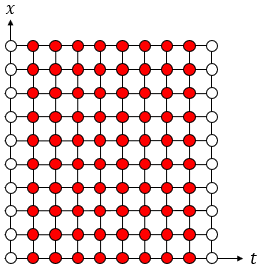
\includegraphics[width=\textwidth]{Boundary.png}
    \caption{Boundary conditions.}
  \end{minipage}
  \begin{minipage}[b]{0.5\textwidth}
    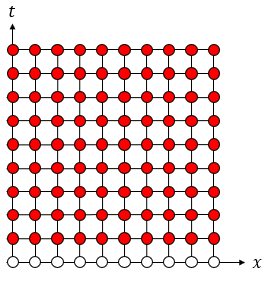
\includegraphics[width=\textwidth]{Initial.png}
    \caption{Initial condition.}
  \end{minipage}
\end{figure}

\subsection{Explicit Method}
Explicit method generalises the parabolic partial differential equation by applying the forward difference to the time derivative and the centred second difference (FTCS).

Applying the finite differences to the parabolic partial differential equation form
\begin{equation}
a(t, x)  u_{xx} + b(t, x) u_x + c(t, x) u_t + d(t, x) u = 0
\end{equation}
\begin{equation}
a(t, x)  \frac{u^n_{i+1}- 2u^n_i + u^n_{i-1}}{(\Delta x)^2}  + b(t, x)  \frac{u^{n}_{i+1} - u^{n}_{i-1}}{\Delta t} + c(t, x)   \frac{u^{n+1}_i - u^n_i}{\Delta t} + d u^n_i = 0
\end{equation}

If we rearrange the formula it can be summarised as
\begin{equation}
u_j^{n+1} = \alpha u_{j-1}^{n} + \beta u_{j}^{n} + \gamma u_{j+1}^{n}
\end{equation}

The formula expresses one unknown nodal value directly in terms of known nodal values  \cite{evans}. Defining $ r = \frac{\Delta t}{\Delta x^2} $. The coefficients for the heat equation becomes
\begin{eqnarray}
\alpha =  r  \\[10pt]
\beta = 1 - 2r  \\[10pt]
\gamma = r  \\[10pt]
\end{eqnarray}

The coefficients for the Black-Scholes partial differential equation becomes
\begin{eqnarray}
\alpha =  \frac{\sigma^2 j^2 \Delta t}{2} - \frac{r j \Delta t}{2} \\[10pt]
\beta = 1 - \sigma^2 j^2 \Delta t - r \Delta t \\[10pt]
\gamma = \frac{\sigma^2 j^2 \Delta t}{2} + \frac{r j \Delta t}{2}
\end{eqnarray}

\begin{figure}[!htb]
    \centering
        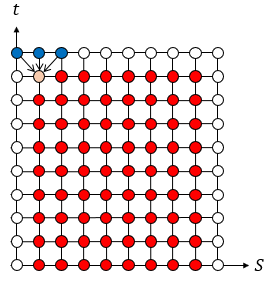
\includegraphics[scale=0.9]{Explicit.png}
    \caption{Computational stencil of explicit method applied to Black-Scholes}
\end{figure}

\subsection{Crank-Nicholson Method}
The explicit method is computationally cheap however this brings a serious drawback, for explicit method to attain reasonable accuracy the step size must be kept small \cite{gdsmith}. Thankfully, the Crank-Nicolson finite difference scheme was introduced by John Crank and Phyllis Nicolson \cite{cn}. Considering numerous articles and publications in the financial engineering literature use Crank-Nicolson as the de-facto scheme for time discretisation, the method has become one of the most popular finite difference schemes for approximating the solution of the Black - Scholes equation and its generalisations \cite{tavella}.

 If we apply backwards time difference instead of forward time difference that Explicit method used and a central space approximation in space again, we get the BTCS scheme. 
 \begin{equation}
 u_t  = a(t, x)  u_{xx} + b(t, x) u_x + c(t, x) u  + d(t, x)
\end{equation}
\begin{equation}
\frac{u^{n+1}_i - u^n_i}{\Delta t}  = a(t, x)  \frac{u^n_{i+1}- 2u^n_i + u^n_{i-1}}{(\Delta x)^2}  + b(t, x)  \frac{u^{n}_i - u^{n-1}_i}{\Delta t}  + c(t, x)  u^n_i + d(t, x)
\end{equation}

In contrast to the FTCS scheme, we now have three unknowns in this equation, the three values of $u$ at the higher time level.  Crank-Nicolson method takes a weighted average of the FTCS and BTCS schemes. Therefore the approximations become
\begin{itemize}
 \item $ u(t,x) \approx \frac{1}{2} ( u^{n+1}_i +  u^n_i) $
 \item $   \frac{\partial u}{\partial t} \approx \frac{u^{n+1}_i - u^n_i}{\Delta t} $
 \item $   \frac{\partial u}{\partial x} \approx \frac{u^n_{i+1} - u^n_{i-1} + u^{n+1}_{i+1} - u^{n+1}_{i-1}}{4\Delta x} $
 \item $ \frac{\partial^2 u}{\partial x^2} \approx \frac{u^n_{i+1}- 2u^n_i + u^n_{i-1} + u^{n+1}_{i+1}- 2u^{n+1}_i + u^{n+1}_{i-1}}{2(\Delta x)^2} $
\end{itemize}

Applying the new finite differences to the parabolic partial differential equation
\begin{multline}
 (-A -B) u^{n+1}_{i+1} + (1 + 2A - C) u^{n+1}_i + (-A + B) u^{n+1}_{i-1} =  \\
=  (A+B) u^{n}_{i+1} + (1 - 2A + C) u^{n}_i + (A - B) u^{n}_{i-1} + D
\end{multline}
$$ A = a(t,x) \frac{\Delta t}{\Delta x^2},  B = b(t,x) \frac{\Delta t}{4\Delta x}, C = c(t,x) \frac{\Delta t}{2},  D = d(t,x) \Delta t $$ 

Note that in contrast to the FTCS scheme, we now have three unknowns in this equation, the three values of $u$ at the higher time level. The left hand side groups the unknowns and the right hand side groups knowns. The system of equations can be represented by a tridiagonal matrix system. This system of equations can be solved by various algorithms such as Gauss elimination or Thomas algorithm.

\subsection{Rannacher Trick}
??

\subsection{Alternating Direction Implicit Method}
The natural extension of our study of the one-dimensional problem would now be to investigate partial differential equations with more than one space-like dimension. When more than one space dimensions are involved, we have to deal with equations such as two dimensional heat equation or multi-asset black-scholes equation. 

\subsubsection{Two Dimensional Heat Equation}
2 Dimensional Heat Equation to test ADI method:
\begin{equation}
\frac{\partial u}{\partial t} = \frac{\partial^2 u}{\partial x^2} +\frac{\partial^2 u}{\partial y^2}
\end{equation}$  $
Initial and boundary condition
\begin{eqnarray}
u(x,y,0) = 1, \hspace{10pt} 0 \leq x \leq x_{\max}, \hspace{10pt} 0 \leq y \leq y_{\max} \\[10pt]
u(x, 0, t) = u(x, y_{max}, t) = 0, \hspace{10pt} 0 \leq t \leq T \\[10pt]
u(x, 0, t) = u(x, 1, t) = 0 , \hspace{10pt} 0 \leq t \leq T
\end{eqnarray}

\begin{definition} Analytical Solution of Two Dimensional Heat Equation
Similarly, applying separation of variables method to the equation
\begin{eqnarray}
u(x,t) = X(x) Y(y) T(t) \\[10pt]
X^{''}(x) - B X(x) = 0 \\[10pt]
Y^{''}(y) - C (y) = 0 \\[10pt]
T^{'}(t) - (B + C) T(t) = 0 \\[10pt]
X(0) = X(1) = 0, \hspace{10pt} Y(0) = Y(1) = 0
\end{eqnarray}

We have solved for X(x) and Y(y) in Analytical Solution of Heat Equation:
\begin{eqnarray} 
X_n (x)=  sin(n \pi x), \hspace{10pt} B = n \pi
Y_m (x)=  sin(m \pi y), \hspace{10pt} C = m \pi
\end{eqnarray}

Solving for $T(t)$ gives the solution
\begin{eqnarray}
T(t) = exp(- \pi \sqrt{m^2 + n^2}) \\[10pt]
u(x, y, t) =\sum_{m=1}^{\infty} \sum_{n=1}^{\infty} A_{mn}  sin(n \pi x) sin(m \pi y) exp(- \pi \sqrt{m^2 + n^2})
\end{eqnarray}

The initial condition gives
\begin{equation}
u(x, y, 0) = 1 = \sum_{m=1}^{\infty} \sum_{n=1}^{\infty}  A_{mn} sin(n \pi x) sin(m \pi y)
\end{equation}
which is a double Fourier sine series. Thus, the coefficient $A_{mn}$ is chosen such that
\begin{equation}
 A_{mn} = 4 \int_{0}^{1}  \int_{0}^{1} sin(\pi n x)  sin(\pi n y) dx dy = \frac{4(cos(\pi n) - 1)(cos(\pi m) - 1)}{\pi^2 m n} 
\end{equation}
Combining the solutions
\begin{multline}
u_{mn}(x, y, t) =  \sum_{m=1}^{\infty} \sum_{n=1}^{\infty} \frac{4(cos(\pi n) - 1)(cos(\pi m) - 1)}{\pi^2 m n}  \\ sin(n \pi x) sin(m \pi y) exp(- \pi \sqrt{m^2 + n^2}) = 0
\end{multline}

\end{definition}


The alternating direction implicit (ADI) method is one of the most common techniques to numerically solve two dimensional parabolic PDEs. ADI schemes give us advantages of implicit finite difference method and computationally only requires to solve tridiagonal matrices.  The scheme was first proposed by Peaceman and Rachford in 1955 for  oil reservoir modelling \cite{peace}. Basically the methods to split the spatial dimensions and solve a 2D problem as two consecutive 1D problems. It is possible to use ADI in more than 3 dimensions which produces the same number of consecutive 1D problems \cite{DougADI}.

In order to develop a more compact notation, we introduce the finite difference operator notation $\delta^2$.
\begin{equation}
\delta x^2 u^{n}_{i,j}  = \frac{u^{n}_{i+1,j} - 2u^{n}_{i,j} + u^{n}_{i-1,j}}{\Delta x^2}
\end{equation}

Explicit approximation of the derivatives can be written as
\begin{equation}
\frac{u^{n+1}_{i,j} + u^{n}_{i,j}}{\Delta t} = \delta x^2 u^{n}_{i,j} + \delta y^2 u^{n}_{i,j}
\end{equation}
Implicit  approximation of the derivatives can be written as
\begin{equation}
\frac{u^{n+1}_{i,j} + u^{n}_{i,j}}{\Delta t} = \delta x^2 u^{n+1}_{i,j} + \delta y^2 u^{n+1}_{i,j}
\end{equation}

Dividing each time step in half we introduce a temporary intermediate unknown $u^{n+1/2}_{i,j}$. Firstly, the two dimensional heat equation is approximating implicitly x and explicitly over y. The total work involved in one time step amounts to solving $ N_{steps} - 1$ tridiagonal systems \cite{morton}. 
\begin{equation}
\frac{u^{n+1/2}_{i,j} + u^{n}_{i,j}}{0.5 \Delta t} = \frac{\delta x^2 u^{n+1/2}_{i,j} }{\Delta x^2} + \frac{\delta y^2 u^{n}_{i,j}}{\Delta y^2}
\end{equation}
Rearranging the set of equations yields a tridiagonal system which is solved for the temporary intermediate unknown $u^{n+1/2}_{i,j}$.
\begin{equation}
- r_x * u^{n+1/2}_{i+1,j} + (1 + 2r_x) u^{n+1/2}_{i,j}  - r_x u^{n+1/2}_{i,j}  = r_y u^{n}_{i,j+1} + (1 + 2r_y) u^{n}_{i,j} + r_y u^{n}_{i,j-1}
\end{equation}

In order to calculate the solution $u^{n+1}_{i,j}$ by approximating explicitly x and implicitly over y.
\begin{equation}
\frac{u^{n+1}_{i,j} + u^{n+1/2}_{i,j}}{0.5 \Delta t} = \frac{\delta x^2 u^{n+1/2}_{i,j} }{\Delta x^2} + \frac{\delta y^2 u^{n+1}_{i,j}}{\Delta y^2}
\end{equation}
Rearranging the set of equations yields a tridiagonal system which can be solved using gaussian elimination, thomas algorithm etc.
\begin{equation}
-r_y u^{n+1}_{i,j+1} + (1 + 2r_y) u^{n+1}_{i,j} - r_y u^{n+1}_{i,j-1} = r_x * u^{n+1/2}_{i+1,j} + (1 + 2r_x) u^{n+1/2}_{i,j} + r_x u^{n+1/2}_{i,j}
\end{equation}

\begin{figure}[!htb]
    \centering
        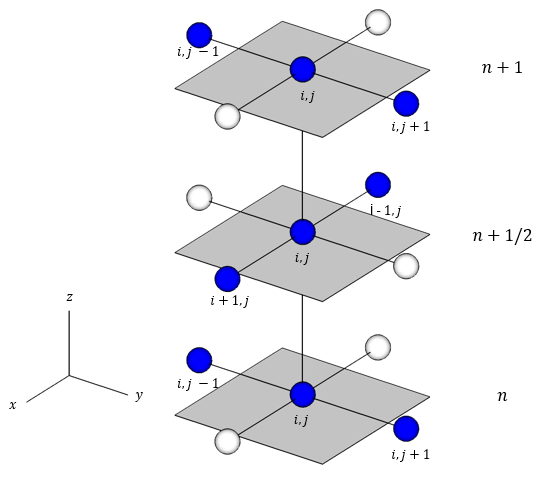
\includegraphics[scale=0.8]{ADI.png}
    \caption{Computational stencil of alternating direction implicit method}
\end{figure}

\chapter{Optimizing Solvers}
Numerical analysis and computer simulations will be undertaken to put theory and observation together to gain insight into the workings of numerical solutions of partial differential equations. First step was deriving toy examples that can be calculated by hand and Excel. Following the verifications, porting the toy examples in C++ and utilize high performance computing principles.

This section documents the performance of attempted optimizations. Experiments  are  conducted  at  W307 computer laboratory, Queen Mary University of London.  Each computer has Windows 10 Enterprise 64 bit, 16 GB of RAM, Intel Core i7-6700 CPU with 4 cores clocked at 3.40 GHz.  The source code is written in C++ and compiled with Microsoft Visual Studio Enterprise 2017, Version 15.3.3 in the release mode. External tools  utilized  in  the  tests  include   Intel Compiler, version 18.0.3 and Intel Math  Kernel  Library, version X .  

\section{Timing the Code}
Measuring execution time intervals accurately is an important aspect to compare the efficiency and speed of different environments and implementations.

\subsection{Windows Application Programming Interface}
Windows Application Programming Interface (API) is the lowest level of interaction between applications and the windows operating system. Thus every program is built upon  the API. Mostly, the interaction is hidden, the runtime and support libraries manage it in the background \cite{windows}. The APIs can be used in the C++ environment. Runtime can be calculated by "QueryPerformanceCounter" or "QueryPerformanceFrequency"  functions. Respectively, the functions retrieve a high resolution time stamp and the frequency of the performance counter. 

\subsection{Chrono Library}
Using the Windows API for just timing the code is slightly excessive given the amount of work it takes. Luckily, Chrono library was introduced part of the C++11’s standard library.  Timers and clocks might differ on distinct systems, thus Chrono library is designed to work effortlessly with date and time. The "high resolution clock" provides the smallest possible tick period and with the “now” method, returns a value corresponding to the call’s point in time.  Once the start and end time of the code is recorded ,  the duration::count method is used to get the elapsed time.

\section{Optimization Experiments}
Main optimization techniques that can be implemented are parallelizing tridiagonal solvers, Visual Studio optimization switches, different compilers and different solution platforms.
\subsection{Tridiagonal Solvers}
Implementing Crank Nicolson and Alternating Direction Implicit methods requires to solve tridiagonal systems which is the most computationally intensive part of the program.  Therefore, choosing efficient tridiagonal solvers is crucial for the speed of the solver. In this experiment three different algorithms will be tested.

\subsubsection{Thomas Algorithm}
Thomas Algorithm is the most commonly used method for solving tridiagonal system of equations. The method is used to solve a tridiagonal matrix system invented by Llewellyn Thomas \cite{thomas}. The system equations can be written as
$$
\begin{bmatrix}  
b_1 & c_1 & 0 & 0 & ... & 0 \\ 
a_2 & b_2 & c_2 & 0 & ... & 0 \\ 
0 & a_3 & b_3 & c_3 & 0 & 0 \\ 
. & . &  &  &  & . \\ 
. & . &  &  &  & . \\ 
. & . &  &  &  & c_{k-1} \\ 
0 & 0 & 0 & 0 & a_k & b_k \\ 
\end{bmatrix} \begin{bmatrix}  
f_1 \\ 
f_2 \\ 
f_3 \\ 
.\\ 
.\\ 
.\\ 
f_k \\ 
\end{bmatrix} = \begin{bmatrix} 
d_1 \\ 
d_2 \\ 
d_3 \\ 
.\\ 
.\\ 
.\\ 
d_k \\ 
\end{bmatrix}
$$

The method begins by forming coefficients \(c^{*}_i\) and \(d^{*}_i\) in place of \(a_i\), \(b_i\) and \(c_i\) as follows:
$$
c^{*}_i = \left\{
     \begin{array}{lr}
       \frac{c_1}{b_1} & ; i = 1\\
       \frac{c_i}{b_i - c^{*}_{i-1} a_i} & ; i = 2,3,...,k-1
     \end{array}
   \right.
$$
$$   
d^{*}_i = \left\{
     \begin{array}{lr}
       \frac{d_1}{b_1} & ; i = 1\\
       \frac{d_i-d^{*}_{i-1} a_i}{b_i - c^{*}_{i-1} a_i} & ; i = 2,3,...,k-1
     \end{array}
   \right.
   $$
With these new coefficients, the matrix equation can be rewritten as:
$$
\begin{bmatrix}  
1 & c^{*}_1 & 0 & 0 & ... & 0 \\ 
0 & 1 & c^{*}_2 & 0 & ... & 0 \\ 
0 & 0 & 1 & c^{*}_3 & 0 & 0 \\ 
. & . &  &  &  & . \\ 
. & . &  &  &  & . \\ 
. & . &  &  &  & c^{*}_{k-1} \\ 
0 & 0 & 0 & 0 & 0 & 1 \\ 
\end{bmatrix} \begin{bmatrix}  
f_1 \\ 
f_2 \\ 
f_3 \\ 
.\\ 
.\\ 
.\\ 
f_k \\ 
\end{bmatrix} = \begin{bmatrix} 
d^{*}_1 \\ 
d^{*}_2 \\ 
d^{*}_3 \\ 
.\\ 
.\\ 
.\\ 
d^{*}_k \\ 
\end{bmatrix}
$$
The algorithm for the solution of these equations is now straightforward and works 'in reverse':

\[ f_k = d^{*}_k, \qquad f_i = d^{*}_k - c^{*}_i x_{i+1}, \qquad i = k-1, k-2, ... ,2,1 \]


 \subsubsection{Intel Math Kernel Library}
 Intel Math Kernel Library implements routines for solving systems of linear equations   from the standard LAPACK library.  Variety of matrix types are supported by the routines. Specifically gtsv function is utilized from the package. Using Gaussian elimination with partial pivoting, gstv computes the solution to the system of linear equations with a tridiagonal coefficient matrix \cite{gtsv}.  
 
 \subsubsection{Cyclic Reduction}
Cyclic reduction was proposed by R. W. Hockney in the 1960s for solving the resulting linear systems from the  discretization of the Poisson equation \cite{Hockney}. 

\subsection{32 bit and 64 bit}
In practical terms, you would use X64 when:  You need to directly address more than 4GB of memory, or   You need very fast (native) processing of 64 bit numerical quantities (including double-precision floating-point numbers) X86 (32 bit) is suitable for most everything else.
    
\subsection{Visual Studio Optimization Switches}


\subsection{Optimal Grid Size}
The resulting analytical solutions are utilised to calculate errors for the solutions using different grid sizes, the grid with the lowest error is used for further tests. Figure X and X demonstrates the error compared to the grid sizes. The optimal grid size for heat equation and Black-Scholes equation is 50 by 50. why uniform olunca daha iyi oluyor araştır??

\begin{figure}[!htb]
  \begin{minipage}[b]{0.5\textwidth}
    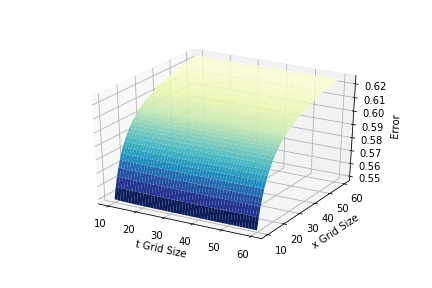
\includegraphics[width=\textwidth]{HeatExplicitGridError.png}
    \caption{Error of grid sizes.}
  \end{minipage}
  \begin{minipage}[b]{0.5\textwidth}
    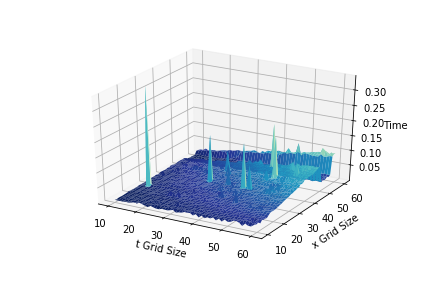
\includegraphics[width=\textwidth]{HeatExplicitGridTimer.png}
    \caption{Timing grid sizes.}
  \end{minipage}
\end{figure}

After choosing the optimal grid size the resulting grids can be visualized as
\begin{figure}[!htb]
  \begin{minipage}[b]{0.5\textwidth}
    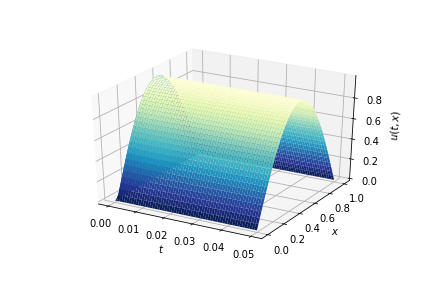
\includegraphics[width=\textwidth]{HeatExplicitGrid.png}
    \caption{Explicit method.}
  \end{minipage}
  \begin{minipage}[b]{0.5\textwidth}
    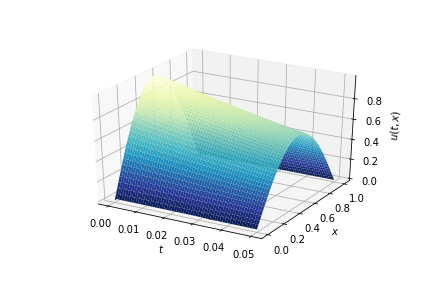
\includegraphics[width=\textwidth]{HeatCNGrid.png}
    \caption{Crank nicolson method.}
  \end{minipage}
\end{figure}

\begin{table}[h!]
\centering
 \begin{tabular}{||c c||} 
 \hline
 Parameter & Value\\ [0.5ex]
 \hline\hline
 Strike Price & 1.0\\ 
 Volatility & 20 \% \\
 Risk Free Rate & 5 \% \\
 Time to Expiry & 2.0\\
 Maximum Share Price & 2.0\\ [1ex] 
 \hline
 \end{tabular}
 \caption{Black-Scholes model testing parameters.}
\end{table}

\begin{table}[h!]
\centering
 \begin{tabular}{||c c||} 
 \hline
 Parameter & Value\\ [0.5ex]
 \hline\hline
  $T$ & 0.075\\ 
  $ x_{max} $  & 1.0  \\ [1ex] 
 \hline
 \end{tabular}
 \caption{One dimensional heat equation testing parameters.}
\end{table}

\begin{table}[h!]
\centering
 \begin{tabular}{||c c||} 
 \hline
 Parameter & Value\\ [0.5ex]
 \hline\hline
  $T$ & 0.075\\ 
  $ x_{max} $  & 1.0  \\ 
   $ y_{max} $  & 1.0  \\ [1ex] 
 \hline
 \end{tabular}
 \caption{Two dimensional heat equation testing parameters.}
\end{table}


\begin{figure}[!htb]
  \begin{minipage}[b]{0.5\textwidth}
    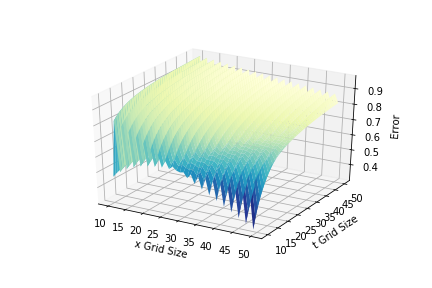
\includegraphics[width=\textwidth]{BSExplicitGridError.png}
    \caption{Error of grid sizes.}
  \end{minipage}
  \begin{minipage}[b]{0.5\textwidth}
    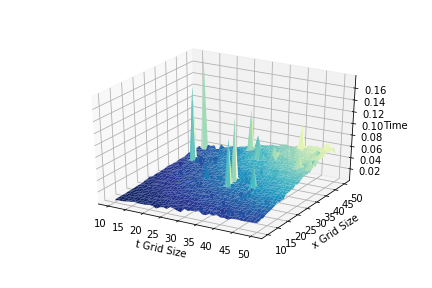
\includegraphics[width=\textwidth]{BSExplicitGridTimer.png}
    \caption{Timing grid sizes.}
  \end{minipage}
\end{figure}

After choosing the optimal grid size the resulting grids can be visualized as
\begin{figure}[!htb]
  \begin{minipage}[b]{0.5\textwidth}
    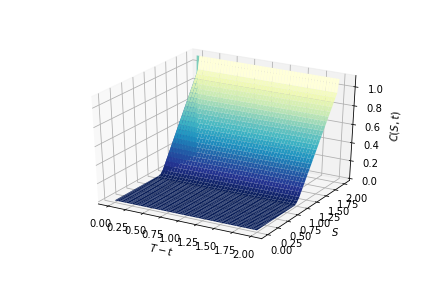
\includegraphics[width=\textwidth]{BSExplicitGrid.png}
    \caption{Explicit method.}
  \end{minipage}
  \begin{minipage}[b]{0.5\textwidth}
    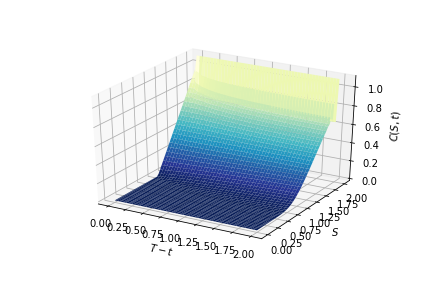
\includegraphics[width=\textwidth]{BSCNGrid.png}
    \caption{Crank nicolson method.}
  \end{minipage}
\end{figure}

\begin{figure}[!htb]
    \centering
        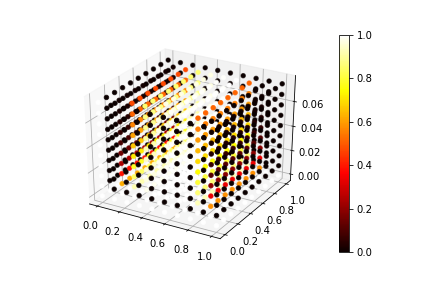
\includegraphics[scale=0.6]{ADIHeat.png}
    \caption{Solution of two dimensional heat equation using ADI.}
\end{figure}

\section{Comparison of methods}
Timing  the tridiagonal systems in a vanilla setup.
Timing  the different compilers and Solution Platforms Timing 32 bit vs 64 bit + VS vs Intel compiler
Timing changing the optimization switches with the most optimal one.

\begin{table}[h!]
\centering
 \begin{tabular}{||c c c||} 
 \hline
 Environment & Explicit Method & Crank Nicolson\\ [0.5ex] 
 \hline\hline\hline
 Visual Studio Compiler x86 & 0.022081 & 0.02035\\ 
 Visual Studio Compiler x64 & 0.018627 & 0.01888\\
 Intel Compiler x86 & 0.023165 & 0.023723\\
 Intel Compiler x64 & 0.019535 & 0.017451\\ [1ex] 
 \hline
 \end{tabular}
 \caption{Averaging 1000 timings for Black-Scholes.}
\end{table}

\begin{table}[htp!]
\centering
 \begin{tabular}{||c c c||} 
 \hline
 Testing & Explicit Method Timing & Crank Nicolson Timing\\ [0.5ex] 
 \hline\hline\hline
 Visual Studio Compiler x86 & 0.022625 & 0.022441\\ 
 Visual Studio Compiler x64 & 0.018933 & 0.016687
\\
 Intel Compiler x86 & 0.023076 & 0.023719\\
 Intel Compiler x64 & 0.017271 & 0.017271\\[1ex] 
 \hline
 \end{tabular}
 \caption{Averaging 1000 timings for Black-Scholes and adding random $\epsilon < 10^{-7} $ to step size in order to avoid compiler optimizations.}
\end{table}
 
\chapter{Conclusions}

\section{Further Work}
aaaaa \cite{fpga},  cloud functions \cite{cloudfunc}.

Threading
High performance computing techniques that can be implemented for multithreading with Open Multi-Processing(OpenMP) and compiler intrinsics.

AVX and Intrinsics
CPUs are pipelining and use of SSE/SIMD kusswurm registers with Advanced Vector Extensions(AVX 512),

GPGPU
 In the case of General Purpose GPUs, CUDA or Open Computing Language(OpenCL) can be utilized but can be challenging because of the requirement of delicate memory management.

\appendix
\chapter{Usage of chrono class}
Should code example be in appendix or stay here?
\begin{verbatim}
auto start = std::chrono::high_resolution_clock::now();
    Portion of code to be timed
auto finish = std::chrono::high_resolution_clock::now();
std::chrono::duration<double> elapsed = finish - start;
std::cout << "Elapsed time: " << elapsed.count() << " s\n";
\end{verbatim}

\chapter{Implementation of the {\tt PDE} class}
Parabolic partial differential equation can be denoted as
$$ \frac{\partial u}{\partial t} = a(t,x) \frac{\partial^2 u}{\partial x^2} + b(t,x) \frac{\partial u}{\partial x} + c(t,x) u(t,x) + d(t,x) $$

$a(t,x)$ denotes diffusion coefficient,  $b(t,x)$ convection coefficient, $c(t,x)$ reaction coefficient, $d(t,x)$ source coefficient
analytic solution, initial conditions boundary conditions
\chapter{Implementation of the {\tt FiniteDifferenceMethod} class}

\begin{verbatim}
void stepSize();
void initialConditions();
void boundaryConditions();
void innerDomain();
void timeMarch();
\end{verbatim}



\bibliographystyle{plain}
\bibliography{ThesisDraft}

\end{document}
